\section{Case Study}
\label{sec:case studies}
We briefly introduce and expand on the concept of driving scenarios to help reason about inherently diverse situations and requirements which an autonomous vehicle might face. 
\begin{figure}[t]
	\centering
	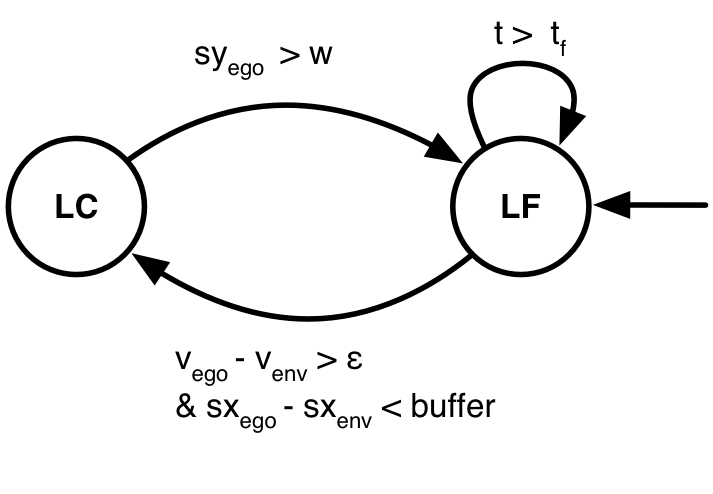
\includegraphics[scale=.6]{figures/behavior_planner}
	\caption{An automaton describing a simplistic behavior planner for lane changes}
	\vspace{-10pt}
	\label{fig:beh planner}
\end{figure}
%In a plan, scenarios are executed and compiled into a sequence known as a mission. 
%In order to satisfy a mission many sequences of scenarios are possible. We aim to show that all of the sequences which might be chosen by the planning level of the controller are safely executed at the lower levels of the controller, and further that sequences might satisfy some higher level properties which indicate the mobility goals of the occupant. The informal idea of scenarios (in the context of driving), can include traffic lights, roundabouts, pedestrians, and even weather conditions. In Scenario \ref{scenario:unsafepassing}, detailed in Figure \ref{fig:danger} we return to the passing scenario as outlined in the introduction. 
\subsection{An unsafe lane change scenario}
The following example describes a lane change scenario in the context of a mission and mobility goals. In this description we imply a valid local planning solution, and seek to verify that all possible individual trajectories which are selected in the \emph{execution} of the plan are safe. First, in \emph{Scenario 1} we will demonstrate a dangerous condition that could have been missed under testing or simulation. Next, in \emph{Scenario 2} we will show how a refinement in the requirements on the perception system or a refinement in the behavioral controller can lead to a provably safe maneuver. Finally, in \emph{Scenario 3} we demonstrate how a change in manufacturer specification can be accurately assessed for safety. To perform verification, we employ dReach version 3.15.10.02 on a Mac OSX laptop with Intel(R) Core i7(R)  2.60GHz CPU and 16 GB memory, and the results are provided in Table~\ref{table:vresults}.

%\begin{figure}[h]
%	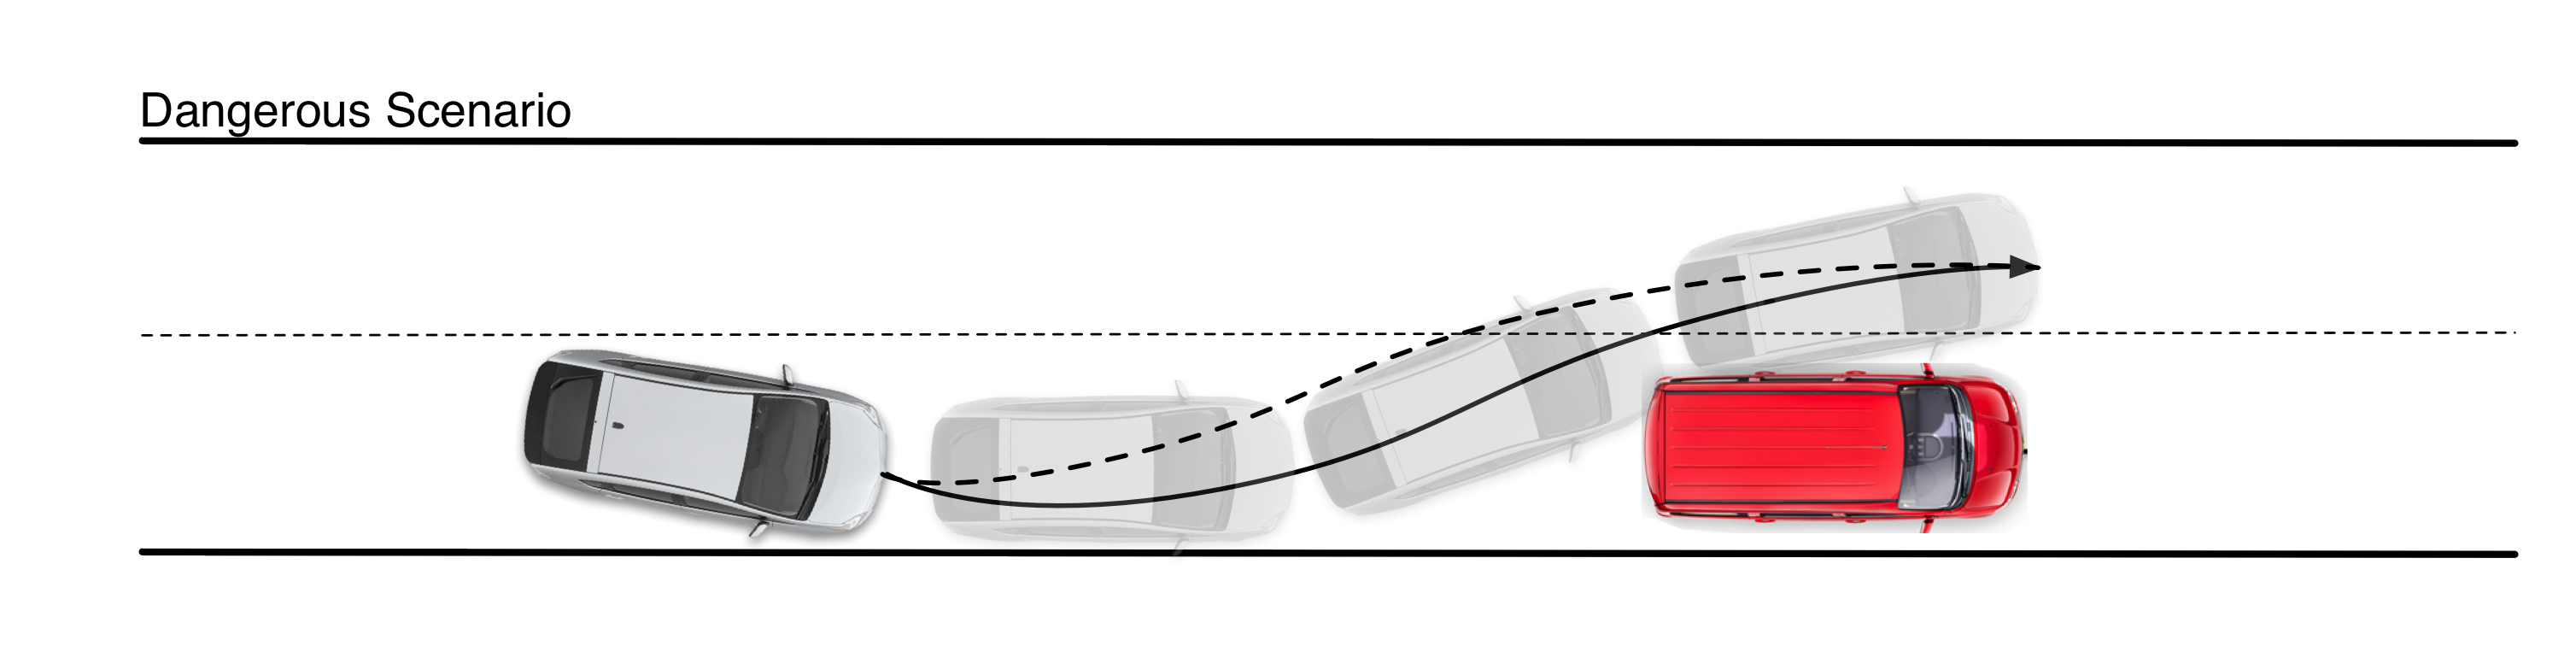
\includegraphics[width=\columnwidth]{figures/danger}
%	\caption{An unsafe lane change scenario that could have been missed in testing due to nonintuitive and uncountably infinite set of initial conditions}
%	\label{fig:danger}
%\end{figure}
%On a typical trip, the autonomous vehicle must recognize, enter, complete and exit many scenarios in a safe and timely manner. 

\begin{figure}[b]
	\vspace{-10pt}
	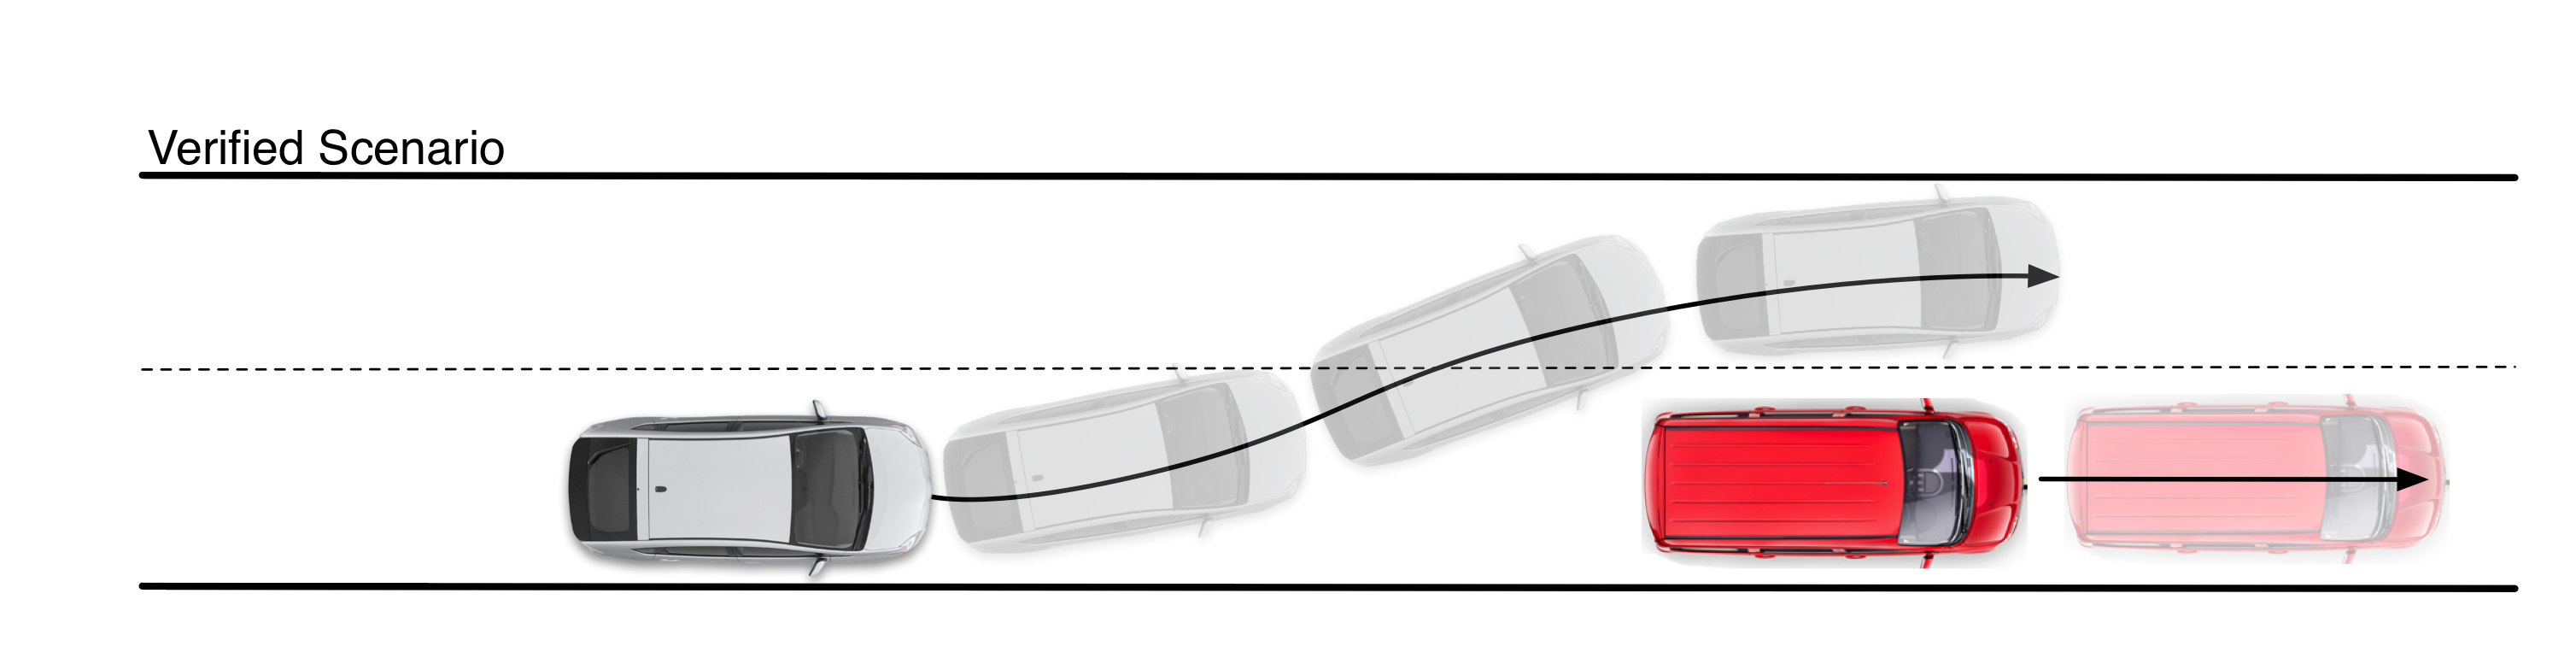
\includegraphics[width=\columnwidth]{figures/safe_scenario}
	\caption{A lane change scenario that could have been missed in testing due to nonintuitive and uncountably infinite set of initial conditions. This scenario is unsafe for certain inter-vehicle buffer spacing and reachability analysis determines the minimum spacing to achieve a safe lance change.}
	\label{fig:danger}
\end{figure}
\vspace{10pt}
\begin{scenario}[{A simple lane change and goal}]
	\label{scenario:unsafepassing}
	As shown in Fig. \ref{fig:danger}, the ego vehicle is driving in the right lane of a uni-directional two lane road network. 
	Another car is driving in front of the ego vehicle at a lower speed. We include the extreme case where the environmental vehicle stops.
	%The ego vehicle's planner must eventually initiate a lane change maneuver, which involves moving to the left lane, in order to enter a left hand turn lane at a four way stop.  
	We highlight that when there is significant uncertainty regarding the ego vehicles orientation and that it may deviate (initially) from the reference trajectory (dashed line) while the tracking controller recovers. We note that the specification of the environment and the ego-vehicle in this scenario are defined as $\xi$ and $\phi$ respectively. \\
\end{scenario}

\subsubsection{Behavioral controller}
We associate a behavioral controller  $\mathcal{B}_1$ with Scenario \ref{scenario:unsafepassing}. 
Figure \ref{fig:beh planner} details the controller, where LC means ``Lane Change" and LF means ``Lane Follow".
Table \ref{table:vresults} records the parameters. It is a simple finite state deterministic automaton. We note, that this particular behavior controller is almost surely too simplistic to cover all of the scenarios faced by an actual vehicle, nevertheless it illustrates how we may formally represent a set of rules which instantiate certain behavior classes on an autonomous vehicle. Similar examples have been published by Darpa Urban Challenge participants \cite{}. Both controllers generated via reinforcement learning and reactive behavior controllers created via synthesis may be represented as deterministic finite automatons. As our current goal is to demonstrate that verification is possible, rather than the richness of the scenarios that the behavioral controller can handle, we find this controller suitable. 

Given any deterministic finite automaton it is possible to express as a \emph{computational logic tree}. Such a tree is rooted in a single state, is infinite in size, and represents a branching notion of time; that is each state (moment in time) may split into multiple possible future worlds. As we will explain in the following sections, such a representation is at the heart of the APEX approach and verification occurs over a bounded search depth on such a computation tree. 

\begin{figure}[h]
	\centering
	\vspace{-10pt}
	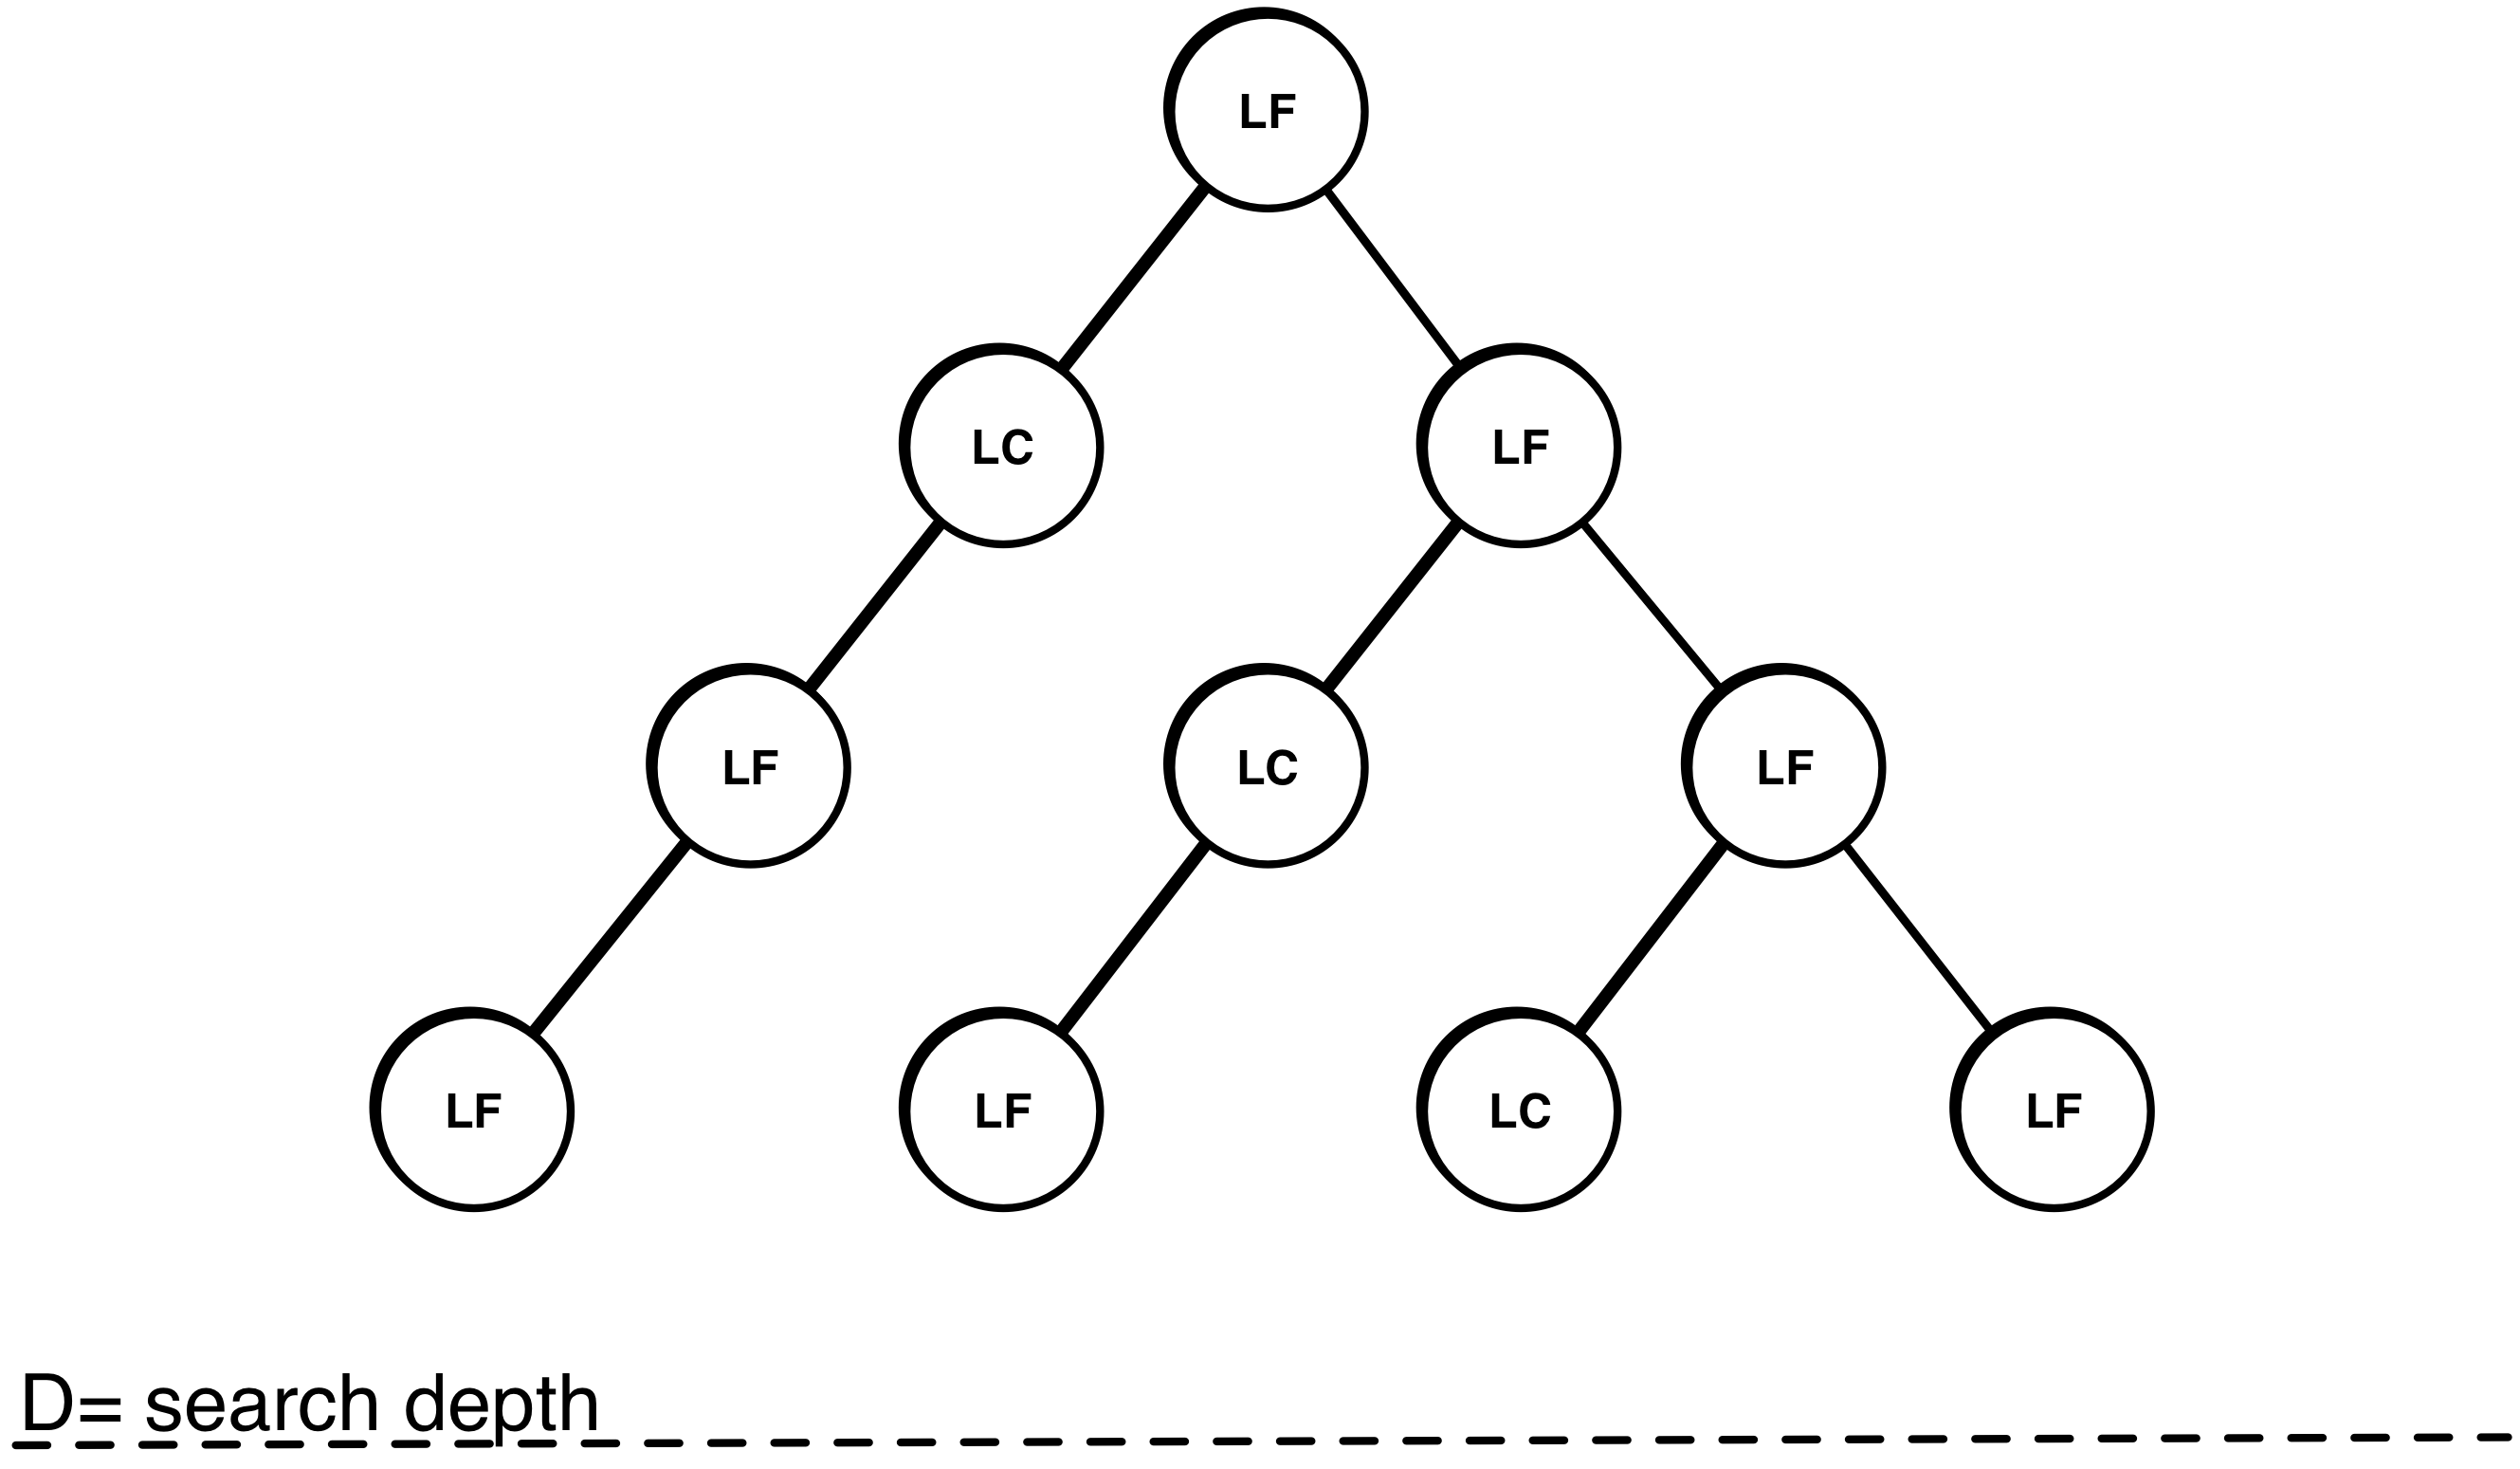
\includegraphics[width=\columnwidth]{figures/exec_tree}
	\caption{An automaton describing a simplistic behavior planner for Lane Following (LF) and Lane Changes (LC)}
	\label{fig:extree}
\end{figure}

We present the initialization of the scenario and the results of the verification. Table \ref{table:vresults} contains the initialization of each parameter.
\subsubsection{Verification and Result}
Finally, for the lane change case, we define an additional constraint set $R_{unsafe}$ as well as a goal set representing the maximum allowable deviation from the goal state. $R_{unsafe}$ expresses that the system fails if it still hasn't changed lanes within 2 sec or it collides with the car ahead of it.
\begin{equation}
\left((s_y<w) \wedge (t>2) \right) \vee \left( (s_y<w) \wedge (sx-\epsilon>s_{x_{env}})\right)
\end{equation}

Then, using APEX we \emph{attempt} to show that there is no execution of the system which can enter $R_{unsafe}$. However, because the system is incorrectly designed dReach returns $\delta$-UNSAFE. 

%\begin{table}[t]
%	\centering
%	\caption{Parameter Initialization Scenario \ref{scenario:unsafepassing}}
	
%	\begin{tabular}{|c|c|}
%		\hline
%		\multicolumn{2}{|c|}{Symbol List} \\ \hline
%		Symbol &  Assignment\\ \hline
%		w & 3.7 m   \\ \hline
%		$\epsilon$ & 1 m/s  \\ \hline
%		buffer & 15 m \\ \hline
%		$t_f$ & 3.0 s \\ \hline
%	\end{tabular}	
%	\label{table:controller_param}
%\end{table}

%\begin{table}[h]
%	\centering
%	\caption{Parameter Initialization Scenario \ref{scenario:unsafepassing}}
%	
%	\begin{tabular}{|c|c|}
%		\hline
%		\multicolumn{2}{|c|}{Symbol List} \\ \hline
%		Symbol &  Assignment\\ \hline
%		$\Psi$ & [0, 0.1]  \\ \hline
%		$v$ & [10.8, 11.1] \\ \hline
%		$s_x$ & [0.0, 0.5] \\ \hline
%		$s_y$ & [0.0, 0.1] \\ \hline
%		$\delta$ & [0.0] \\ \hline
%		$\kappa$ &[0.0] \\ \hline
%	\end{tabular}	
%	\label{table:unsafetable}
%\end{table}

\subsection{A safe lane change scenario}
Using the information and counterexample from the previous scenario it is easy to see that the behavior controller must be corrected in order to guarantee safety of the lane change scenario. 
\begin{scenario}[{A more conservative behavioral controller}]
	\label{scenario:safepassing}
	We begin with Scenario \ref{scenario:unsafepassing}.
	In order to ensure the forward safety of the vehicle we propose a small modification to the behavioral controller of the vehicle, and furthermore require that the ego vehicle's localization system return estimates with less uncertainty. 
	Namely, we first increase the size of variable buffer, so that the ego vehicle is forced to initiate a lane change maneuver earlier.
	Secondly, we decrease the size of the initial sets.
	Speed $v$ now starts anywhere in $[10.9,11]$ and $s_y$ starts in [0.0,0.05].\\
\end{scenario}

With these changes, dReal returns SAFE, meaning that no trajectory of the system violates the constraints.

\begin{table}[]
	\centering
	\caption{Verification Results}
	\begin{tabular}{|l|l|l|l|}
		\hline
		Symbol & Scenario 1 & Scenario 2 & Scenario 3 \\ \hline
		$w$ & 3.7 & 3.7 & 3.7 \\ \hline
		$B$ & 15 & 20 & 20 \\ \hline
		$\delta$ & 0.1 & 0.1 & 0.1 \\ \hline
		$v_{ego}$ & [10.8, 11.1] & [10.9, 11] & [10.9, 11] \\ \hline
		$s_{x_{ego}}$ & [0.0, 0.5] & [0.0, 0.5] & [0.0, 0.5] \\ \hline
		$s_{y_{ego}}$ & [0.0, 0.1] & [0.0, 0.05] & [0.0, 0.05] \\ \hline
		$\Psi$ & [0.0, 0.1] & [0.0, 0.1] & [0.0, 0.2] \\ \hline
		Search Depth & 2 & 2 & 2 \\ \hline
		Verification Time (s) & 30.821 & 373.924 & 36.166 \\ \hline
		Result & $\delta$-UNSAFE & SAFE & $\delta$-UNSAFE \\ \hline
	\end{tabular}
	\label{table:vresults}
\end{table}

\subsection{A supplier issues a specification change}
Given that a safe controller has been found a supplier wishes to know if they may reduce the accuracy of several key sensors associated with localization of the ego vehicle. Such a specification change is known to add significant uncertainty to the estimate of the ego vehicle's heading angle during the planning phase. 

\begin{scenario}[{Large perception errors}]
	\label{scenario:perception}
	We begin with Scenario \ref{scenario:safepassing}.
	In order to reflect the change in supplier specification we update the localization system return estimates to reflect greater uncertainty. 
	Namely, we increase the size of the intial set for ego vehicle heading such that $\Psi$ starts in [0.0,0.2].\\
\end{scenario}

The result of this modification is again $\delta$-UNSAFE, because the ego vehicle clips the rear bumper of the environmental vehicle while executing the lane change maneuver. Again the engineer in charge of the project may use the new information to refine the controller design or reject the suppliers specification change. In this way formal verification efforts can be a useful tool in determining the \emph{requirements} which sensors and perception systems must meet given a particular control algorithm. 

%\subsection{Building an Overtaking Maneuver}
%Part II: Overtake\begin{itemize}
%	\item Ego, antagonist, and discrete lane blockage variable
%	\item Safety properties: don't crash and speed
%	\item Liveness properties: Get around slow vehicle within x amount of time...
%\end{itemize}

%\subsection{Results}
%\begin{itemize}
%	\item Show safety of planned trajectories in first order logic
%	\item Show verification of each world (BDD path to leaf) in LTL
%	\item List time to verify
	
%\end{itemize}